\chapter{Probabilistic SCast}

% **************************** Define Graphics Path **************************
    \graphicspath{{Chapter5-PSCast/Figs/Vector/}{Chapter5-PSCast/Figs/}}

This chapter explores the consequences of utilising the \textsf{ABcast} protocol for state machine replication between $s$-nodes in the \textsf{AmaaS} model.  Throughout our explanations we assume that the \textsf{SCast} protocol and its system model are utilised for all interactions between $c$-nodes and the ordering service.  We refer to this approach as Probabilistic \textsf{SCast}, or \textsf{PSCast} for short. 

The remainder of this chapter is structured as follows: First we present the new \emph{amcast} guarantees provided by \textsf{PSCast}.  We then explore the ramifications of these new guarantees and discuss how they can cause \emph{amcast} messages to be delivered out of the total order at one or more destinations.  Finally, we describe the consequences of such missorderings, within the context of Infinispan, and explore potential solutions that can be employed by Infinispan to tolerate these missorderings.  

\newpage
\section{PSCast Guarantees}
Below, we state the \emph{amcast} guarantees provided by \textsf{PSCast}.  
   
    \begin{description}
        \item [\textbf{G1}] - \emph{Validity}: If the source of $m_i$ does not crash until it \emph{abcast}s $m_i$, then all operative destinations of $m_i$ deliver $m_i$.
       
        \item [\textbf{G2}] - \emph{Uniform Agreement}: If the source of $m_i$ crashes while \emph{abcast}ing $m_i$, and if any destination delivers $m_i$, then all operative
destinations of $m_i$ must deliver $m_i$.
        
        \item [\textbf{G3}] - \emph{Uniform Integrity}: If $m_i$ has already been delivered by a destination $d$, then $d$ cannot deliver $m_i$ again.  
       
        \item [\textbf{G4-PSCast}] - \emph{Probabilistic Total Order}: If two \emph{\emph{amcast}s}, $m_i$ and $m_j$, have common destinations, then all such destinations that deliver both $m_i$ and $m_j$, will deliver them in an identical order with a probability $> R$.  Typically $R \rightarrow 1$.
\end{description}

\textbf{Note:} The guarantees of \textsf{PSCast} are identical to those of the underlying \emph{abcast} protocol, \textsf{ABcast}.  This is because the guarantees of the \emph{abcast} protocol, and any violations of these guarantees, directly impacts how each $s$-node maintains its $order\_history[]$ and generates $m.history[]$; with $m.history[]$ dictating the order in which a $c$-node must deliver \emph{amcast}s ($\S$ \ref{sec:scast_protocol}).  

\section{G4-PSCast Violations}
Recall that the \textsf{SCast} protocol utilises the final timestamp of the \emph{abcast} message, which contains a clients ordering request, to determine the total order of the \emph{amcast}.  

The \textsf{SCast} protocol, described in chapter \ref{ch:amaas}, assumes that the underlying \emph{abcast} protocol provides deterministic guarantees for all G1-G4 ($\S$ \ref{sec:atomic_guarantees}).  Hence, the \textsf{SCast} protocol assumes that all $s$-nodes will eventually deliver an \emph{abcast} and that all \emph{abcast}s are delivered in the same order at each destination.  This assumption means that the \textsf{SCast} protocol is able to guarantee that all \emph{amcast}s sent via the ordering service will respect G4 as it is guaranteed that all $s$-nodes will always maintain a consistent $order\_history[]$.  Therefore, all ordering responses, $rsp(Tx)$, from the service will contain the correct $m.history[]$ data.  

Conversely, \textsf{PSCast} utilises a probabilistic \emph{abcast} protocol, \textsf{ABcast}, that only guarantees G4 with probability $R$ (G4-P).  Therefore, for an \emph{abcast} $m$ sent between $s$-nodes, there is a small probability ($1-R$) that a destination, $N_s$, will not receive or \emph{know} of $m$ after $\Delta_m$ time.  In this case, it is possible for another \emph{abcast}, $m'$, $m.ts < m'.ts$, sent from a different $s$-node, $m.o \neq m'.o$, to have been delivered at $N_s$ when $\Delta_m'$ expired.  Resulting in a violation of G4-P, as $m'$ has preceded $m$, which causes $N_s$ to \emph{reject} $m$ from the total order and deliver it to the application (\textsf{SCast}), via an exception, when it eventually arrives.  

This G4-P violation, and hence the \emph{late} delivery of $m$, can be abstracted as follows: For every message, $m$, that is about to be added to the $ordering\_history[]$, a random value, $RV$, is assigned, which is uniformly distributed between $0$ and $1$.  $RV$ is then compared with the probability that G4-P will hold, $R$, before $m$ is added to the $ordering\_history[]$. Two cases are then possible:

    \begin{description}
        \item[$\bm{RV \leq R}$]\hfill \\
        This represents that G4-P was met and therefore $m$ is processed the same as in the deterministic \textsf{SCast} protocol.  Hence, $m$ is added to a node's $order\_history[]$ instantly as described in \textsf{SCast}.  
        
        \item[$\bm{RV > R}$]\hfill \\
        This represents that G4-P was not met, as G4-P is guaranteed with probability $R$.  In this case, $m$ is not inserted in $order\_history[]$ before $x$ time; with $x$ being a random time in the future, which represents the unknown time at which $m$ would be delivered via an exception at the node that did not maintain G4-P.  Consequently, subsequent \emph{abcast} messages, $m'$, $m'.ts > m.ts$, delivered by this node before $x$, are inserted into $order\_history[]$ ahead of $m$.  
    \end{description}
    
    By the way of comparison, we now explore the consequences of a message being assigned $RV > R$, with respect to the $order\_history[]$ and $m.history[]$ generated by an $s$-node.  Consider a scenario where an $s$-node receives four \emph{abcast}s, $\{m_1, m_2, m_3, m_4\}$; where each $m$ corresponds to a transaction with the same value, \emph{e.g.} $m_1 \rightarrow Tx_1$, and $m_1.dst = \{C_1, C_2, C_3\}; m_2.dst = \{C_1, C_3\}; m_3.dst = \{C_1, C_2\}; m_4 = \{C_2, C_3\}$.  Furthermore, each $mcast(Tx_1)$ message sent as per the \textsf{SCast} protocol, is denoted as $mc_1$ for short, \emph{e.g.} $mc_1$ is associated with the same \emph{amcast} as $Tx_1$ and $m_1$.  
    
    If all four messages are allocated an $RV$ value, $RV \leq R$, then all messages are inserted into the $order\_history[]$ in the correct order.  Therefore, a correct $m_4.history[]$ is produced by this node; the resulting $order\_history[]$ and $m_4.history[]$ generated upon delivery of $m_4$ are shown in Figure \ref{fig:correct_ohistory_pscast}.  
    
    Alternatively, consider that a single message, $m_3$, is allocated a value $RV > R$.  This causes $m_3$ to be delayed for $x$ time.  Assuming that $m_4$ is delivered before $x$ time, $m_4$ will take $m_3$'s place in the total order, resulting in an erroneous $order\_history[]$ and $m_4.history[]$.  This is shown in Figure \ref{fig:incorrect_ohistory_pscast}.  
    
    \begin{figure}[h] 
        \centering
         \makebox[\textwidth][c]{\includegraphics[width=1.25\textwidth]{correct_ohistory}}
         \caption[Order History with deterministic ordering (G4)]{$order\_history[]$ with deterministic ordering (G4)}
         \label{fig:correct_ohistory_pscast}
    \end{figure}    

    \begin{figure}[h] 
        \centering
         \makebox[\textwidth][c]{\includegraphics[width=1.25\textwidth]{wrong_ohistory}}
         \caption[Order History with non-deterministic ordering (G4-P is not met)]{$order\_history[]$ with non-deterministic ordering (G4-P is not met)}
         \label{fig:incorrect_ohistory_pscast}
    \end{figure}  
    
    The consequences of the incorrect $m_4.history[]$, as shown in Figure \ref{fig:incorrect_ohistory_pscast}, are that it is now possible for the $c$-node, $N_c2$, to miss $mc_3$ in its total order, even though ${mc_3 \ \llcurly_{N_c2} \ mc_4}$.  In order for such a miss-ordering to occur, both of the following must be true:
    
    \begin{enumerate}[label=\roman*]
        \item $N_c2$ \textbf{\emph{receives}} $mc_4$ before $mc_3$.     
        
        \item $N_c2$ \textbf{\emph{delivers}} the message stated in $mc_4.history[N_c2]$ before receiving $mc_3$.  
    \end{enumerate}
    
    If condition $(i)$ is true, then $N_c2$ will not know of $mc_3$ as it is not stated in $mc_4.history[]$ and if $(ii)$ is also true, then $mc_4$ will be delivered immediately.  Note, that if $N_c2$ was to receive $mc_3$, before delivering $mc_4.history[Nc_2]$, then $mc_3$ will be \emph{known} by $Nc_2$ and the correct delivery order of ${mc_1 \ \llcurly_{Nc_2} \ mc_3 \ \llcurly_{Nc_2} \ mc_4}$ will be preserved.  

    \textbf{Note:} The probability of a G4-PSCast violation is the product of two probabilities; the probability that a G4-P violation occurs, \emph{i.e.} $R$; and the probability that both conditions $(i)$ and $(ii)$ are met.  Therefore, in practice the probability of a G4-PSCast violation occurring is much smaller than $(1 - R)$.  

\section{Service Node - Mitigating G4-P Violations}
In the previous section we defined how violations of G4-P occur and the consequences of such occurrences on \textsf{PSCast} (G4-PSCast violations).  We now explore how G4-P violations can be handled by $s$-nodes in order to reduce the chances of G4-PSCast violations from occurring.  

Let $m$ be an \emph{abcast} sent between $s$-nodes and $m'$ be a subsequent \emph{abcast}, where $m \llcurly_d m'$ for all $d \in tx.dst \cap tx'.dst$; where $tx$ and $tx'$ are the transactions associated with \emph{abcast}s $m$ and $m'$ respectively.  Now consider that $m$ is assigned a value $RV > R$ and $m'$ $RV \leq R$ at an $s$-node $N_s$.  In such circumstances two possibilities exist:

    \begin{enumerate}
        \item    $N_s$ delivers $m'$ before delivering $m$ via an exception.
        
        \item    $N_s$ delivers $m$ via an exception, before $m'$ is received and delivered.  
    \end{enumerate}
    
    In scenario $(i)$, $N_s$ $order\_history[]$ will be missing $m$ when $m'.history[]$ is calculated, therefore it is \emph{possible} for one or more $d$ to suffer from a G4-PSCast violation.  In this case, it is not possible for $N_s$ to update $order\_history[d]$ as it already stores the latest message associated with $d$, $m'.ts$ and $m \llcurly_d m'$.  However, it is necessary for $N_s$ to update $order\_history[d'] \forall d' \in m.dst \setminus m'.dst$ as subsequent messages, $m''$, involving $d'$, where $m \llcurly_{d'} m''$, require $m$ to be specified in $order\_history[d']$ in order to create a valid $m''.history[d']$ \footnote{If a message stored in $order\_history[d']$ is greater than $m.ts$, \emph{i.e.} $m \prec_d' order\_history[d']$, then $m$ is ignored for this entry.  Such a scenario is possible if $m \prec m'$, opposed to $m \llcurly m'$, and a subsequent \emph{abcast} involving $d'$ is delivered at $N_s$ before the exception containing $m$.}.   
    
    Scenario $(ii)$, is handled the same as $(i)$, except that we know that the entries for $order\_history[d]$ will be correct for all $d$ as $m$ has been delivered to $N_s$ before $m'$.  

    \textbf{Note:} If none of the above actions were taken, the $order\_history[]$ would eventually correct itself, \emph{i.e.} preventing invalid $.history[]$ being generated, as eventually a new message, $\bar{m}$, would be received for each $c$-node in the network; where $\tilde{c}$ represents all $c$-nodes and $order\_history[\tilde{c}] \prec \bar{m}$; hence $order\_history[\tilde{c}]$ is set to $\bar{m}$.  The only scenario where a $c$-node, say $c$'s, entry in $order\_history[c]$ would not eventually be corrected is when no subsequent ordering requests are received which specify $c$ as a destination.  However, in such a scenario the $order\_history[c]$ entry would never be used again, hence this invalid entry cannot cause any G4-PSCast violations.  
    
    \paragraph{Crash-Tolerance} \hfill \\
    In scenario $(i)$ described above, it is not possible for $m$ to create a correct $m.history[]$ as $m'$ will be present in $order\_history[d] \forall d \in m.dst \cap m'.dst$.  However, an accurate $m.history[]$ needs to be generated in order to store a local copy of $m$, at $N_s$, as it may be required in the event of a crashed node ($\S$ \ref{ssec:scast_fault_tolerance} $C3$ and $S1-S4$).  A possible solution to this problem, is to utilise a partially-persistent version of $order\_history[]$, $\bar{order}\_\bar{history}[]$, that allows past values associated with a given $c$-node to be queried \footnote{This could be implemented by maintaining a partially-persistent linked list for each client, with each subsequent message associated with a client simply appended to the end of the list.}.  This would enable $N_s$ to query $\bar{order}\_\bar{history}[d] \forall d \in m.dst$ and find the message that precedes $m$ in the total order so that it can create an accurate $m.history[]$.
    
    A limitation of such an approach would be the amount of memory consumed by the $\bar{order}\_\bar{history}[]$ data structure, however this is not a major concern as the amount of data required for each message is very small.  Therefore, utilising an eviction scheme alongside reusable data objects would allow such a scheme to function indefinitely whilst storing thousands of message records at any one time.  

\section{Client Nodes - Detecting G4-PSCast Violations}
Recall that \textsf{SCast} utilises a single \emph{delivery} thread to process the AWQ and $am\_deliver()$ all \emph{amcast} messages ($mcast()$) to the application.  In addition to these threads, we also assume there exists several \emph{worker} threads which are responsible for delivering and processing unicast messages to the \textsf{SCast} protocol.  It is these threads that process unicast messages and determine whether they are $mcast()$ messages which must be added to the AWQ or if they are unicast messages required by higher-level protocols in the stack; in which case, the \emph{worker} threads simply forwards the messages up the stack \footnote{The \emph{delivery} thread is not required as normal unicast messages do not adhere to a total order}.  

To detect G4-PSCast violations, we modify the behaviour of the original \textsf{SCast} protocol.  Instead of placing all received $mcast()$ messages into the AWQ, it is now necessary for the \emph{worker} thread to inspect the $mcast()$ message, $m$, and determine whether $m$ has missed its place in the total order.  This is achieved by comparing $m.order$ with $last\_amcast.order$; where $last\_amcast$ is the last $mcast()$ message that invoked $am\_deliver()$.  If $last\_amcast.order \prec m.order$, then $m$ can be added to the AWQ and processed as normal.  However, if $m.order \prec last\_amcast.order$ then we know that $m$ has been missed in this node's total order, therefore it is necessary for the primitive $am\_deliver\_with\_exception()$ to be invoked.  

The purpose of $am\_deliver\_with\_exception()$ is to enable an the application to still receive $m$, whilst being aware that a G4-PSCast violation has occurred.  Assuming that the primitive has been invoked for a $mcast()$ $m$, $am\_deliver\_with\_exception()$ works as follows:  $m$ is assigned an error bit to identify it as a G4-PSCast violation and it is delivered to the application via a \emph{worker} thread, \emph{i.e.} as a normal unicast message.  The \emph{delivery} thread is not utilised as this node's total order has already been violated and it is necessary for the higher level application to receive $m$ as soon as possible.  

For example, let \emph{amcast}'s $m_1 \prec_d m_2$ for a $c$-node destination $d$.  Now assume that a G4-P violation occurred at an $s$-node when processing $m_1$, which results in $m_2.history[]$ missing $m_1$ for $m_2.history[d]$.  Let $d$ receive and deliver $m_2$, before eventually receiving $m_1$; hence $last\_amcast = m_2$.  Upon receiving $m_1$, $d$ will realise that $m_1 \prec last\_amcast$ and will therefore invoke $am\_deliver\_with\_exception(m_1)$.  Assuming that the application is still executing $m_2$ using the \emph{delivery} thread, it is possible for the application to receive $m_1$ via a \emph{worker} thread and initiate a recovery mechanism  as soon as possible, in order to counteract $m_1$'s G4-PSCast violation.  

The pseudocode for receving a message and determining whether a $mcast()$ has suffered a G4-PSCast violation at a destination $d$ is presented in Algorithm \ref{ps:detect_g4pscast}, whilst the pseudocode for processing the AWQ remains the same as Algorithm \ref{ps:awq} presented in section \ref{sec:scast_protocol}.  

    \begin{algorithm}[H]
       \caption{PSCast Receive Message}
        \label{ps:detect_g4pscast}
        \begin{algorithmic}[1]
	        \STATE{$m \leftarrow receive\_message();$}
	        \IF{$m$ is $mcast()$}
		         \IF{$last\_amcast \prec_d m.order$}
		                \STATE{$add\_to\_AWQ(m);$}
		         \ELSIF{$m.order \prec_d last\_amcast$}
		                \STATE{$am\_deliver\_with\_exception(m);$}
		         \ENDIF
		     \ELSE
		         \STATE{$forward\_to\_application(m);$}
		     \ENDIF
        \end{algorithmic}
    \end{algorithm}   

\section{Infinispan (Client Node) - Mitigating G4-PSCast Violations}
% Transaction manager, state all assumptions - exceptions etc.
    In the event that one or more G4-PSCast violations occur, it is necessary for the client application to be able to recover from such events.  In this subsection, we present a recovery mechanism that can be employed by the Infinispan transaction manager at each $c$-node in the event of a violation occurring.  The exact methods of the recovery mechanism are determined by the isolation level chosen by the Infinispan clients before runtime; with one method required for \emph{Repeatable Read}, $RR$ and \emph{Read Committed}, $RC$ transactions, whilst an alternative method is required for $RR$ with WSC due to its dependence on a voting phase to commit/abort transactions.  Therefore, we first explored the method required for $RR$ and $RC$ before detailing the provisions for $RR$ with WSC.  
    
    \subsection{Transaction Manager Assumptions}
    Our solutions for recovering from G4-PSCast violations assume that the following data structures are implemented by the Transaction Manager (TM):
    
    \begin{description}
        \item[$\bm{tx\_entry}$] \hfill \\
        For a transaction, $Tx$, the following data must be stored:
            \begin{itemize}
                \item    The duration of the transaction from its inception. $(\bm{Tx.duration})$.            
            
                \item    A boolean flag, which is set to true if $Tx$ was delivered to the TM via an exception.  $(\bm{Tx.exceptional})$.
            
                \item    The value of all $(k,v)$ pairs in this $Tx$ at the time $Tx$ starts to be processed. $(\bm{Tx.start\_pairs})$.
                
                \item    The $m.order$ value associated with the \emph{amcast} which delivered $Tx$'s $prepare(Tx)$ message.  $(\bm{Tx.order})$.
                
                \item    The final decision, whether to \emph{abort} or \emph{commit} the transaction. $(\bm{Tx.decision})$.
                
                \item    A an associative array of all $commit()$ or $abort()$ votes received for this transaction, with the source destination of a vote being used for indexing ($RR$ with $WSC$ \emph{only}).  $(Tx.votes[])$. \textbf{Note:} votes received for transactions that have not yet been processed by a TM are stored in a temporary buffer until the associated transaction becomes active; at which point the votes are \emph{received} and added to $Tx.votes[]$.  
            \end{itemize}
            
        Henceforth, all references to a transaction, or $Tx$, assumes that a $tx\_entry$ is maintained along with all of the above values.  
            
        \item[$\bm{tx\_queue}$] \hfill \\
        The transaction queue, $tx\_queue$, is a priority queue which stores the TM's currently executing transaction, $Tx$, as its head entry; a $Tx$ is dequeued when it has finished executing and pushed onto $tx\_history$.  Subsequent entries in the queue are additional transactions, $Tx'$ that proceed $Tx$ in the total order.  \textbf{Note:} When no G4-PSCast violations have occurred, the $tx\_queue$ should only contain $Tx$.  
        
        \item[$\bm{tx\_history}$] \hfill \\
        The transaction history, $tx\_history$, is a stack which stores the transactions which have already been committed by the TM, with the $Tx$ stored at the top of the stack representing the last transaction to have been committed by the TM.  
    \end{description}
    
    \subsubsection*{Delivery Thread and TM}
    As the \emph{delivery} thread utilised by \textsf{PSCast} is responsible for delivering all $mcast()$ messages that do not suffer a G4-PSCast violation, we assume that this thread is also responsible for processing the $tx\_queue$ upon message delivery.  Therefore, transaction processing occurs as follows: At the \textsf{PSCast} level when $am\_deliver()$ is invoked, the \emph{delivery} thread passes the $prepare(Tx)$ message upto the TM, adds the $Tx$ to $tx\_queue$ and starts processing $tx\_queue$; hence $Tx$.  Once all messages in the $tx\_queue$ have been processed, the \emph{delivery} thread returns to the \textsf{PSCast} level and starts processing the next message in \textsf{SCast}'s AWQ.
    
    \subsubsection*{Worker Threads and TM}
    We assume that all unicast messages sent between TMs are delivered up their destination's network stack and to their local TM via a \emph{worker} thread.  This enables the TM to receive unicast messages from other TMs, \emph{e.g.} votes when WSC is enabled, whilst enabling the \emph{delivery} thread to be utilised solely for \emph{amcast}s that require processing by the TM.  
       
    \subsection{Repeatable Read and Read Committed} \label{ssec:rr_rc_recovery}
    When $RR$ or $RC$ isolation is utilised the outcome of a transaction is determined in a single phase as each $d \in Tx.dst$ deterministically decides whether to commit or abort a transaction without requiring any additional communication between destinations.  Consequently, when a TM receives a $prepare(Tx)$ message via \textsf{PSCast}, assuming that G4-PSCast holds, the TM is able to commit the transaction immediately.  
    
    Now consider that an \emph{amcast} $prepare(Tx)$ message, $m_i$ has violated G4-PSCast and a subsequent \emph{amcast} $m_j$ has been delivered to the TM before $m_i$.  In such a scenario, the TM remains unaware of $m_i$ until $am\_deliver\_with\_exception(m_i)$ has been called by the \textsf{PSCast} layer below and $m_i$ is received via an exception.  Therefore, until TM receives such an exception, the transaction associated with $m_j$ and any other $m$ delivered ahead of $m_i$ will be processed as if no G4-PSCast violation has occurred.  
    
    When $m_i$ is delivered to the TM via an exception, the only course of action is for a roll-back procedure, similar to that utilised in compensating transactions \citep{Korth:1990:FAR:645916.671971}, to be initiated; with all transactions that should have been executed after $m_i$'s transaction being reversed.  Once all of the offending transactions have been reversed it is possible for $m_i$'s transaction to be executed and the previously rolled back transactions reapplied in the correct total order.  Hence, the data maintained by this $c$-node eventually becomes the same as if no G4-PSCast violation had occurred.  
    
    For example, if the original value of a key $k$ was $v=5$, the transaction associated with $m_i$ was $put(k, 10)$ and $m_j$'s transaction was $put(k, v+1)$.  When $m_i$ is missing, the outcome of $m_j$'s transaction would be $v = 6$, however after $m_i$ is delivered via an exception and the transactions are re-executed, the result of $m_j$'s transaction will be $v = 11$.  
    
    \subsubsection*{TM roll-back Implementation}
    Assume the same scenario as described in the previous section, with $m_j$ being incorrectly delivered to the TM ahead of $m_i$; where $m_j$ and $m_i$ are associated with transactions $Tx_j$ and $Tx_i$ respectively.  When a destination eventually receives $m_i$, it invokes $am\_deliver\_with\_exception(m_i)$ and delivers $m_i$ to the TM using the \emph{worker} thread which delivered $m_i$ to the \textsf{PSCast} layer.  Upon receiving $m_i$, and hence $Tx_i$, the TM takes the following actions:
    
    \begin{enumerate}
        \item    $Tx_i$ is stored within the TM as a $tx\_entry$ and inserted into the $tx\_queue$.  An interrupt is sent to the \emph{delivery} thread so that it is aware that at least one $Tx$ exists in the queue.  
        
        \item    The \emph{delivery} thread finishes executing its current transaction before processing the next $Tx$ in the $tx\_queue$; which will most likely be $Tx_i$ \footnote{Assuming only one G4-PSCast violation occurs, $Tx_i$ will always be inserted at the head of the queue.}.
        
        \item    During the execution of $Tx_i$, past transactions stored in $tx\_history$ are \emph{popped} from $tx\_history$ and inserted into the $tx\_queue$ (in order), until no transactions exist in $tx\_history$ which precede $Tx_i$ in the total order.
        
        \item    Once all of the required transactions have been (re-)inserted into $tx\_queue$, the TM will execute $Tx_i$ and then push $Tx_i$ onto $tx\_history$.  This process continues until the $tx\_queue$ becomes empty, at which point all transactions that are known by the TM will have been executed in the order dictated by \textsf{PSCast}.  
        
        \item    Once the $tx\_queue$ becomes empty, the roll-back procedure is considered complete and the \emph{delivery} thread is able to return to the \textsf{PSCast} level to start processing the next \emph{amcast} message in the AWQ.  
    \end{enumerate}        
    
    Figure \ref{fig:tx_queue_history}, shows the process of a transaction $tx_3$ being executed and then pushed onto $tx\_history$.  Note how $tx_2$ is missing from $tx\_history$ as it was missed in the total order.  Figure \ref{fig:tx_queue_history_rollback} shows the roll-back procedure being executed once $tx_2$ is delivered to the TM via an exception, with $tx_3$ being popped from $tx\_history$, as it was erroneously executed ahead of $tx_2$, and reinserted into the $tx\_queue$ in its correct order behind $tx_2$.  
    
    \begin{figure}[h] 
        \centering
         \makebox[\textwidth][c]{\includegraphics[width=.75\textwidth]{tx_queue}}
         \caption[TM $tx\_queue$ and $tx\_history$]{TM $tx\_queue$ and $tx\_history$}
         \label{fig:tx_queue_history}
    \end{figure}      
    
    \begin{figure}[h] 
        \centering
         \makebox[\textwidth][c]{\includegraphics[width=.9\textwidth]{tx_queue_rollback}}
         \caption[TM $tx\_queue$ and $tx\_history$ Executing a Roll-back]{TM $tx\_queue$ and $tx\_history$ Executing a Roll-back}
         \label{fig:tx_queue_history_rollback}
    \end{figure}  
    
    Algorithm \ref{ps:tx_queue_rr_rc} outlines the steps required by the TM to process the $tx\_queue$ when Repeatable Read or Read Committed isolation is utilised by transactions.  In this algorithm, we assume that the transaction associated with the interrupting exception has already been added to $tx\_queue$.  
    
    \begin{algorithm}[H]
        \caption{TM $tx\_queue$ Processing for RR and RC Isolation}
        \label{ps:tx_queue_rr_rc}
        \begin{algorithmic}[1]
            \WHILE{$tx\_queue$ is not empty}
                \STATE{$tx \leftarrow dequeue(tx\_queue);$}
                \STATE{$previous\_tx \leftarrow pop(tx\_history);$}
                
                \WHILE{$tx \prec previous\_tx$}
                    \STATE{$insert\_into\_tx\_queue(previous\_tx);$}
                    \STATE{$previous\_tx \leftarrow pop(tx\_history);$}
                    \STATE{$revert\_commit(previous\_tx);$}
                \ENDWHILE
                             
                \IF{$previous\_tx \prec tx$ $\land$ $previous\_tx$ is not $null$}
                    \STATE{$push\_to\_tx\_history(previous\_tx);$}
                \ENDIF
                
                \STATE{$tx.decision \leftarrow process(tx);$}   
                \IF{$tx.decision \neq abort(tx)$}
                    \STATE{$push\_to\_tx\_history(tx);$}
                \ENDIF
                
                \STATE{$execute(tx)$;}
            \ENDWHILE
        \end{algorithmic}%
    \end{algorithm}
    
    \subsubsection*{Limitations}
    A consequence of utilising a roll-back mechanism, with $RR$ or $RC$ isolation, is that \textquoteleft{}stale' reads can occur as it is possible for a subsequent transaction, to read $v = 6$ when requesting the value of $k$, ultimately leading to \emph{write-skew}.  We consider this an acceptable risk for three reasons: 
    \begin{enumerate}[label=\roman*]
        \item    G4-PSCast violations are already the product of several small probabilities, therefore the probability of \emph{write-skew} occurring is even smaller.  
        
        \item    The window of opportunity for a \emph{write-skew} to occur is very small.  We anticipate that the time between a G4-PSCast violation occurring and being detected to be in the order of milliseconds.   
        
        \item    The Infinispan store is already susceptible to \emph{write-skew}s when the WSC is not utilised, therefore the business logic of the application utilising Infinispan should already be tolerant of such phenomena.  
    \end{enumerate}    
    
    \subsection{Repeatable Read with WSC}
        % Present Solution with pseudocode
        % Provide examples and figures of the interesting cases and discuss how are solution works
        
        When utilising transactions with $RR$ and WSC it is not possible to just utilise the roll-back procedure outlined in section \ref{ssec:rr_rc_recovery}, as the outcome of each transaction affects the second voting phase that is required to avoid \emph{write-skews}.  However, the additional voting stage required by the WSC can be used to our advantage to prevent G4-PSCast violations from affecting the consistency of Infinispan's key/values.  
        
        Recall that the WSC requires that a transaction coordinator, $Tx.c$, receives at least one commit vote for each of the distinct keys involved in a $Tx$ in order for it to be able to send a final $commit(Tx)$ decision to all $Tx.dst$.  Whereas, $Tx.c$ only requires a single abort vote from any of the $Tx.dst$ members in order to disseminate an $abort(Tx)$ decision.  Furthermore, for every key stored in the infinispan system there exists a single \emph{primary} replica and at least one \emph{backup} replica.  The solutions presented in this section require a slight modification to this existing WSC behaviour.  Our solutions require that: 

\begin{quotation}    
    For all transactions, votes to commit or abort a transaction can only be sent by the transaction manager of the client node which contains the \emph{primary} replica of a key.  
\end{quotation}

    Again consider that an \emph{amcast} $prepare(Tx)$ message, $m_i$ has violated G4-PSCast and a subsequent \emph{amcast} $m_j$ has been delivered to the TM before $m_i$.  As is the case for RR and RC isolation, the TM only becomes aware of $m_i$ once $am\_deliver\_with\_exception(m_i)$ has been called by the \textsf{PSCast} layer.  Upon receiving $m_i$, its associated transaction, $tx_i$ is inserted into $tx\_queue$.  In the event that the \emph{delivery} thread is currently processing another $Tx$, $tx_i$ is not processed until $Tx$ has finished executing.  
    
    \subsubsection*{TM Classification}    
    How each $Tx$ stored in $tx\_queue$ is processed, depends entirely on the $(k,v)$ pairs involved in an individual $Tx$ and the relationship of the TM with each of these pairs.  Below we define three classifications of TM with respect to an individual $Tx$:
    
    \begin{description}
        \item[\emph{Primary} TM] \hfill \\
            We classify a TM as being a \emph{primary} for a given $Tx$, if this node hosts a \emph{primary} replica of one or more $(k,v)$ pairs that are modified by this transaction.  Read requests do not count, as these actions have already been performed before the $prepare(Tx)$ message was \emph{amcast}.  
            
        \item[\emph{Backup} TM] \hfill \\
        A TM is classified as a \emph{backup}, if it only hosts \emph{backup} replicas of the $(k, v)$ pairs involved in a $Tx$.  A TM cannot be a \emph{backup} if it hosts a \emph{primary} replica of any of the $(k,v)$ in the $Tx$.  
        
        \item[\emph{Coordinator} TM] \hfill \\
        A TM is classifed as the \emph{coordinator}, if the node hosting the TM was the original node who initiated $Tx$, \emph{i.e.} $Tx.c$, or if this node is the currently active coordinator for the $Tx$, \emph{i.e.} $Tx.\tilde{c}$.  
    \end{description}
    
    \textbf{Note:} It is possible for a TM to be both a \emph{coordinator} and a \emph{primary} or a \emph{coordinator} and \emph{backup}, simultaneously.  However, by definition it is not possible for a TM to be both a \emph{primary} and a \emph{backup}.
    
    \subsubsection*{Processing a Transaction}
    Once a $Tx$ becomes the head of $tx\_queue$, and hence the active transaction, it is passed to the function $process(Tx)$ which determines whether $Tx$ should be committed or aborted.  The actions taken by the TM when executing $process(Tx)$ depends on its classification, therefore we present the actions of each classification below:
    
    \begin{description}
        \item[\emph{Primary} TM] \hfill \\
        A \emph{primary} TM takes the following actions for a $Tx$:
            \begin{enumerate}
                \item[1a.]    If $Tx$ was delivered via exception, \emph{i.e.} $tx.exceptional$ is true, then send an abort $vote(Tx)$ to $Tx.c$
                
                \item[1b.]    Otherwise, the outcome of the write skew check determines the vote to be sent to $Tx.c$, either $commit(tx)$ or $abort(tx)$.  
                
                \item[2.]    Wait to receive the final decision from the $Tx.c$.  
            \end{enumerate}
            
        \item[\emph{Backup} TM] \hfill \\
         As \emph{backup} TM does not vote towards the progress of a transaction, it simply waits to receive a final decision for $Tx$ from the $Tx.c$.  
        
        \item[\emph{Coordinator} TM] \hfill \\
        If a \emph{coordinator} is also a \emph{primary} then it is necessary for the \emph{coordinator} to first cast a vote as required by the \emph{primary} TM role before executing the actions required by a \emph{coordinator}.  A \emph{coordinator} must take the following actions:
        
        \begin{enumerate}
            \item[1.]    Wait to receive a vote from all \emph{primary} TMs associated with $Tx$.  
            
            \item[2a.]    If a single $abort(Tx)$ vote is received, then stop waiting and send an final $abort(Tx)$ decision to all $d \in Tx.dst$.  
            
            \item[2b.]    Otherwise, if a $commit(Tx)$ is received from all \emph{primaries}, send a final $commit(Tx)$ decision to all $d \in Tx.dst$.  
        \end{enumerate}
        
        \textbf{Note:} If a single $abort(Tx)$ vote, or all $commit()$ votes, are not received after a pre-determined timeout period then the \emph{coordinator} aborts $Tx$.  This abort timeout is necessary to overcome a deadlock scenario which, although unlikely, is possible with our solution.  This deadlock scenario is explored in detail later on in this section.  
    \end{description}              
    
    Once a $Tx$ has been processed and a final decision established, it is necessary for it to be removed from $tx\_queue$ and the decision enacted.  If the $Tx$ is to be committed, it must also be pushed to $tx\_history$.  At this point the execution of $Tx$ at the local TM is complete, and the next $Tx'$ in $tx\_queue$ can be processed.  
    
    Algorithms \ref{ps:tx_queue_rr_wsc} and \ref{ps:transaction_manager_process_tx} present the pseudocode for processing $tx\_queue$ and executing $process(tx)$, respectively, when WSC is enabled.  The purpose of lines 5-15 in Algorithm \ref{ps:transaction_manager_process_tx} is described in the next section.  
    
    \begin{algorithm}
        \caption{Transaction Manager RR with WSC $tx\_queue$ Processing}
        \label{ps:tx_queue_rr_wsc}
        \begin{algorithmic}[1]
            \WHILE{$tx\_queue$ is not empty}
                \STATE{$tx \leftarrow peek(tx\_queue);$}
                \STATE{$tx.decision \leftarrow process(tx);$}
                
                \IF{$tx.decision \neq abort(tx)$}
                    \IF{Not a primary for any $(k,v)$ in $tx$}
                        %roll-back
                        \STATE{$previous\_tx \leftarrow pop(tx\_history);$}
		                 \WHILE{$tx \prec previous\_tx$}
		                     \STATE{$insert\_into\_tx\_queue(previous\_tx);$}
		                     \STATE{$previous\_tx \leftarrow pop(tx\_history);$}
		                     \STATE{$revert\_commit(previous\_tx);$}
		                 \ENDWHILE
		                 
		                 \IF{$previous\_tx \prec tx$ $\land$ $previous\_tx$ is not $null$}
                            \STATE{$push\_to\_tx\_history(previous\_tx);$}
                        \ENDIF
                    \ENDIF
                    \STATE{$push\_to\_tx\_history(tx);$}
                \ENDIF
                \STATE{$dequeue(tx\_queue);$}
                \STATE{$execute(tx)$;}
            \ENDWHILE
        \end{algorithmic}%
    \end{algorithm}

    \begin{algorithm}
        \caption{TM $process(tx)$ with WSC}
        \label{ps:transaction_manager_process_tx}
        \begin{algorithmic}[1]
            \IF{TM hosts $primary$ replica of any $(k,v)$ in $tx$}
                \IF{$tx.exceptional$ is true}
	                \STATE{$v \leftarrow abort(tx);$}
                \ELSE
	                \STATE{$v \leftarrow write\_skew\_check();$}
	            \ENDIF
	            \STATE{$send\_vote(v);$}
            \ENDIF
            \\
            \IF{TM is $tx$ Coordinator}
	            \STATE{$votes\_rec \leftarrow size(tx.votes[]);$}
	            \WHILE{$votes\_rec < \#primaries$ in $tx.dst$}
	                \IF{$tx.duration$ $>$ $timeout$}
	                    \STATE{$decision \leftarrow abort(tx);$}
	                    \STATE{\textbf{break};}
	                \ELSE
	                    \STATE{$v \leftarrow receive\_vote();$}
		                \STATE{$tx.votes[source\_address(v)] \leftarrow v;$}
		                \IF{$v$ = $abort(tx)$}
		                    \STATE{$decision \leftarrow abort(tx);$}
		                \ENDIF
	                \ENDIF
	            \ENDWHILE
	            \IF{$descision$ is not set}
	                \STATE{$decision \leftarrow commit(tx);$}
	            \ENDIF
	            \STATE{send $decision$ to all $d \in tx.dst;$}
	        \ENDIF
	        \\
	        \STATE{$tx.decision \leftarrow receive\_final\_decision();$}
	        \RETURN{$tx.decision$}
        \end{algorithmic}
    \end{algorithm}
    
        \subsubsection*{\emph{Backup} TM Roll-back Required}
        Previously we stated that it was not possible to utilise the roll-back procedure utilised by RR and RC isolation when the WSC was enabled.  This is true when a TM is classified as a \emph{primary}, however in the case of a \emph{backup} TM it is possible, and sometimes required, for a roll-back mechanism to be utilised.  The roll-back mechanism detailed on lines 5-15 of Algorithm \ref{ps:tx_queue_rr_wsc} functions in much the same way as when RR or RC isolation is utilised and is required in the following scenario:
        
        Let $m_i$ and $m_j$, contain the transactions $tx_i$ and $tx_j$ respectively, where $m_i \prec m_j$.  Assume that both $tx_i$ and $tx_j$ consist of a single write operation, $put(k1,x)$ \footnote{We assume that the value of $x$ is different for each $Tx$}, where nodes $N_c1$ and $N_c2$ host the \emph{primary} and \emph{backup} replica of $k1$, respectively.  Finally, assume that node $N_c3$ is the $Tx.c$ for $tx_i$ and $N_c4$ is the $Tx.c$ for $tx_j$. 
        
        Let $m_i$ and $m_j$ be successfully delivered at $N_c1$, resulting in the \emph{primary} TM ($N_c1$) processing $Tx_i$ and $Tx_j$ in the correct order.  Let, $N_c3$ and $N_c4$ receive $m_i$ and $m_j$ respectively, without any G4-PSCast violations. Now consider that $m_i$ suffers a G4-PSCast violation at its backup node, $N_c2$, and $m_j$ is delivered ahead of it in the total order.  This results in $N_c2$'s active transaction being $tx_j$.  
        
        Consequently, $tx_i$ is the active transaction for its coordinator and all of its \emph{primary} TMs, therefore it is guaranteed that a final decision for $tx_i$ will be reached and eventually sent to $N_c2$'s TM.  As $N_c2$'s active $Tx$ is $tx_j$, $N_c2$ will not process $tx_i$'s final decision until $tx_j$ has finished executing.  Therefore, $N_c2$'s TM will execute $tx_j$ before $tx_i$, whereas $k$'s \emph{primary} TM $N_c1$ will have executed $tx_i$ before $tx_j$.  Thus, the \emph{backup} replica of $k$ has become inconsistent from the \emph{primary} replica.  \textbf{Note:} An inconsistency only occurs at the \emph{backup} TM if the final decision for both $tx_i$ and $tx_j$ is commit.  
        
        Figure \ref{fig:wsc_backup_rollback} shows the message flow required by all parties in order for the above scenario to occur.  
        
    \begin{figure}[h] 
        \centering
         \makebox[\textwidth][c]{\includegraphics[width=1.25\textwidth]{backup_rollback}}
         \caption[\textsf{PSCast}: Roll-back Scenario with WSC]{\textsf{PSCast}: Roll-back Scenario with WSC}
         \label{fig:wsc_backup_rollback}
    \end{figure}    
        
        
        When an inconsistency occurs between a \emph{backup} and \emph{primary} replica as described above, it is possible to perform a roll-back operation at the \emph{backup} node as the \emph{backup} node does not influence the coordinator's decision to commit/abort a transaction.  Hence, performing a roll-back operation on a \emph{backup} node is the same as when RR or RC isolation is utilised.  
        
        
        \subsubsection*{Deadlock Scenario}
    Let $N_c1$ and $N_c2$ be the \emph{primary} replica for $k1$ and $k2$, respectively.  Assume that \emph{amcast}s $m_i$ and $m_j$ correspond to transactions $tx_i$ and $tx_j$, with both transactions having $N_c3$ as their coordinator and the following operations included in their payload: 
    
    \begin{lstlisting}
	    Tx.begin();
		    put(k1, x);
		    put(k2, y);
		Tx.commit();
    \end{lstlisting}
    
    Assume that $m_i$ and $m_j$ are both successfully delivered at $N_c1$ and $N_c3$, resulting in both of their TM's setting $tx_i$ as their active transaction.  Now assume that $m_j$ is delivered ahead of $m_i$ at $N_c2$ due to a G4-PSCast violation;  resulting in $N_c2$'s TM having $tx_j$ as its active transaction.  
    
    Such a scenario results in a deadlock occurring between the two transactions, as the \emph{coordinator}, who is executing $tx_i$ will be waiting indefinitely for a vote from $N_c2$.  This vote will never arrive from $N_c2$ as its current transaction is $tx_j$, hence only a vote for $tx_j$ will be sent to $tx_j.c$.  Figure \ref{fig:wsc_deadlock} shows the message flow required for deadlock to occur.  
    
    \begin{figure}[h] 
        \centering
         \makebox[\textwidth][c]{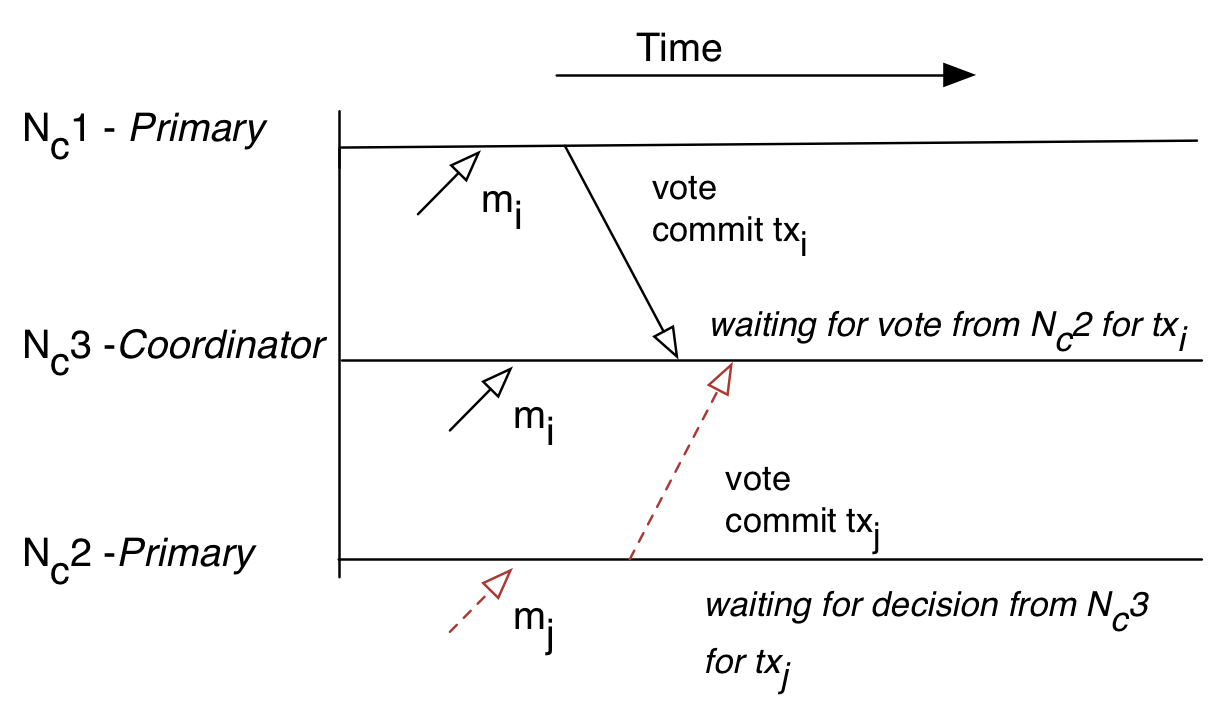
\includegraphics[width=\textwidth]{deadlock_wsc}}
         \caption[\textsf{PSCast}: Deadlock Scenario with WSC]{\textsf{PSCast}: Deadlock Scenario with WSC}
         \label{fig:wsc_deadlock}
    \end{figure}       
    
    To prevent such a deadlock from halting progress indefinitely we introduce an abort timeout as per the Two-phase commit protocol ($\S$ \ref{ssec:2PC}).  Therefore, in the case described above, $tx_i$ will eventually abort as no progress can be made until $tx_i$ timesout at $N_c3$.
    
    \textbf{Note:} Although we have reintroduced deadlock into the total order commit protocol, such occurrences are very rare.  The probability of a transaction being aborted is equal to the probability of a G4-PSCast violation occurring at a \emph{primary} TM when a $Tx$ involves multiple keys whose \emph{primary} replicas exists across several nodes.  

\section{Summary}
In this chapter we have explored the consequences of utilising the \textsf{ABcast} protocol for state machine replication between $s$-nodes in the \textsf{AmaaS} model; which we refer to as \textsf{PSCast}.  We explore the consequences of \textsf{ABcast}'s probabilistic guarantees not being met between $s$-nodes, specifically G4-PSCast violations at client nodes, and potential strategies for overcoming such violations.  More specifically, we have provided an in-depth exploration of potential strategies that could be adopted by Infinispan's transaction manager's to ensure that the consistency of its key/value pairs is maintained.  